
\documentclass[runningheads]{llncs}
\usepackage{amssymb, bm, mathtools}
\usepackage{subcaption}
\usepackage[pdftex, xetex]{graphicx}
\usepackage{enumerate, setspace}
\usepackage{float, colortbl, tabularx, longtable, multirow, subcaption, environ, wrapfig, textcomp, booktabs}
\usepackage{pgf, tikz, framed, url, hyperref}
\usepackage[normalem]{ulem}
\usetikzlibrary{arrows,positioning,automata,shadows,fit,shapes}
\usepackage[english]{babel}
\usepackage{listings}
\usepackage{microtype}
\usepackage{times}
\usepackage{algorithm}
\usepackage{algpseudocode}
\usepackage{pifont}
\usepackage{graphicx,verbatimbox}
\usepackage{wrapfig}
\usepackage{lipsum}
\usepackage{fontawesome5}
\usepackage{hyperref}

\begin{document}
\title{Boosting Few-Shot Meta Q-Learning with Reptile Optimization Algorithm}
\author{Spandan Rout\inst{1}\and
Milinda Basavaraju\inst{2}\and
Nithish Balu\inst{3}}

\authorrunning{M. Tanya et al.}

\institute{\email{spandanrout@icloud.com} \and
\email{miluvarsha@gmail.com} \and
\email{nithishmoritz@gmail.com}}

\maketitle

\section{Introduction}
Highly complex computational models excel when ample training data is available and despite their computational intensity, the training process can be notably protracted. In contrast, human cognition exhibits rapid learning and the ability to make extrapolations based on only a scant amount of data. The challenge of effective learning under data scarcity remains a critical issue in the realm of computational intelligence. In this study, we seek to empirically validate the efficacy of few-shot learning within the domain of decision-making optimization. Through experimentation within a simulated control environment, we aim to showcase the potential of this approach. The full details of our project's implementation can be accessed through the provided link: \url{https://github.com/sheilsarda/ESE546_Final_Project} 

\section{Background}
Meta-learning is the machine learning field pertaining to the problem of ``learning how to learn." Few-shot learning is the sub-field that addresses how a machine can learn when only given a few samples. Traditionally, a computational system undergoes extensive familiarization on a suite of closely related computational challenges and subsequently encounters a distinct yet related challenge, with access to only a limited number of novel data points. Essentially, the objective of few-shot learning revolves around enabling robust generalization when constrained to take merely a few $k$ gradient descent steps. There have been three major approaches for few-shot learning:

\begin{enumerate}
	\item Using prior knowledge about similarity: Whereas ML models cannot discriminate between classes not present in the training data, few-shot learning enables models to separate classes that are not present, allowing the models to separate unseen classes. Examples of this include Siamese Networks (discriminating two unseen classes) \cite{koch2015siamese} and Matching Networks (discriminating multiple unseen classes) \cite{vinyals2016matching}.
	
	\item Exploiting prior knowledge: By using the structure and variability of the data, models can generalize recurring patterns. This is especially prevalent in computer vision tasks like object detection \cite{lake2015human}.
	
	\item Constraining the learning algorithm: By choosing specific hyperparameters or choosing learning update rules that converge quickly, few-shot learning enables models to generalize well on small amounts of training data. Examples of these include Reptile \cite{nichol2018first} (an application of the Shortest Descent algorithm) and SNAIL \cite{mishra2017simple} (which uses temporal convolutions to aggregate contextual information). 
	
\end{enumerate}

\noindent The third approach is the focus of our study. Typically, such few-shot learning algorithms are general; they only specify the way in which gradient updates are made. In the case of the Algorithm-M for Rapid Adaptation (AMRA), the researchers were able to generalize the algorithm to work on regression, classification, and reinforcement learning problems, and showed it working on MiniImageNet and Mujoco's HalfCheetah and Ant environments \cite{finn17maml}. MAML presented a problem, however, in that it required Hessian computations, rendering it an intensive algorithm for machines with limited memory and power. Subsequent studies such as the first-order MAML (FOMAML) and Reptile tried to alleviate this problem by taking an initial linear estimation of the Hessian matrix and computing the average stochastic gradient across all tasks. While Reptile showed promising results for classification using the Omniglot and MiniImageNet datasets and CNN models, the researchers showed ``negative results” on Reinforcement Learning \cite{nichol2018first}. This presents an opportunity to apply Reptile on reinforcement learning tasks. Recent developments in this field have also studied the effect of weight sharing based on the ordering of the tasks across time \cite{riemer2019learning}.


\section{Approach}
The goal of our project is to understand and explore
limited-data adaptability within the Decision Optimization domain. At first, we tried to replicate the MAML paper by running Mujoco's HalfCheetah and Ant environments. However, we found the task too computationally complex and time-intensive, since the task was in continuous space. Thus, to implement few-shot learning, we used OpenAI Gym's CartPole environment. We then built and trained a Deep Q-Network on a set of related tasks and asked the model to generalize its learning on a hold-out set of tasks based on a few training steps.

\subsection{Simulation Environments} 

We modified OpenAI Gym's CartPole environment to create unique but related simulations. The Pendulum-Cart System, consists of a pole connected to a mobile cart via a passive linkage mechanism. This system operates on a smooth, low-friction track. Initially, the system is in an unstable state, necessitating training to enable the control mechanism to manage the pole's balance. Control is achieved by applying a directional force of +1 or -1 to the cart, with the objective being to maintain the pole's vertical position. Performance is evaluated through a continuous reward mechanism, and episodes terminate under specific conditions. By varying the gravity and pole mass, different but related tasks were created. Attached is a summary of the simulation environments:

\begin{table}[H]
\centering
\begin{tabular}{|l|c|c|c|c|}
\hline
\rowcolor[HTML]{000000} 
{\color[HTML]{FFFFFF} Environment Name} &
  \multicolumn{1}{l|}{\cellcolor[HTML]{000000}{\color[HTML]{FFFFFF} Max Episode Steps}} &
  \multicolumn{1}{l|}{\cellcolor[HTML]{000000}{\color[HTML]{FFFFFF} Reward Threshold}} &
  \multicolumn{1}{l|}{\cellcolor[HTML]{000000}{\color[HTML]{FFFFFF} Standard Gravity (g)}} &
  \multicolumn{1}{l|}{\cellcolor[HTML]{000000}{\color[HTML]{FFFFFF} Mass of Pole (kg)}} \\ \hline
CartPole-v0  & 200 & 195 & 9.8 & 0.1 \\ \hline
CartPole-v2  & 200 & 195 & 20  & 0.1 \\ \hline
CartPole-v3  & 200 & 195 & 30  & 0.1 \\ \hline
CartPole-v4  & 200 & 195 & 40  & 0.1 \\ \hline
CartPole-v5  & 200 & 195 & 50  & 0.1 \\ \hline
CartPole-v6  & 200 & 195 & 60  & 0.1 \\ \hline
CartPole-v7  & 200 & 195 & 10  & 0.2 \\ \hline
CartPole-v8  & 200 & 195 & 10  & 0.4 \\ \hline
CartPole-v9  & 200 & 195 & 10  & 0.8 \\ \hline
CartPole-v10 & 200 & 195 & 10  & 1.0 \\ \hline
\end{tabular}
\end{table}

\noindent Our Deep Q-Network model was trained randomly on a subset of the above tasks, with the exception of  CartPole-v6 and CartPole-v10, which were held out as a validation set to test our few-shot learning implementation.

\subsection{Neural Network Architecture} 
\subsubsection{Deep Q Networks}
Advanced Q-Optimization is a conventional model-independent technique within the domain of Decision Optimization. Given a Q-function: $S \times A \rightarrow \mathbb{R}$, we can construct a policy that maximizes our long-term rewards:
$$\pi = \underset{a}{argmax}q(s,a)$$  
For large state or action spaces, a non-linear function approximator like a neural network can be useful. Then, we establish an update rule based on the Bellman equation: 
$$q(s,a) = R_{t+1}(s,a) + \gamma max_{a}q(s_{t+1}, a_{t+1})$$
However, the use of non-linear function approximators to represent the Q-function introduces instabilities in the model. These instabilities stem from correlations between the target value and the actual Q-function estimates. To achieve an ideal policy, our objective is the minimization of the $L^1$ divergence between the q-function estimation and the target Q-value $\hat{y}(s,a)$:
$$loss = Q(s,a) - \hat{y}(s,a)$$  
To reduce these instabilities, methods like experience replay introduce a replay buffer. With a replay buffer, it is then possible to collect prior transitions $\{s, a_i, s^{'}, R(s,a)\}$  and sample from prior transitions before any updates are made. 

\subsubsection{Parameters} 
We use the following DQN with 3 fully connected layers to play over the various CartPole environments: 
\begin{verbbox}[\small]
# ______ DQN PARAMS ______ # 
GAMMA = 0.99 
BATCH_SIZE = 16
memory_replay = Replay_Buffer(10000) 
episodes = 500 
target_updates = 10

state_dim = 4
action_dim = 2 
h_dim1 = 64
h_dim2 = 256

# ______ REPTILE HYERPARAMETERS______ # 
meta_step_size_final = .1
meta_step_size = .1 
k_iters = 200 # Tunable  
\end{verbbox}
    \begin{figure}[h!]
  \centering
  \theverbbox\qquad
  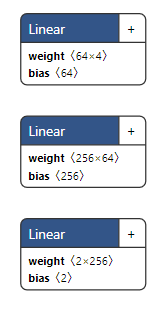
\includegraphics[scale=.5]{architecture_diagram.png}
  \caption{Deep Q-Network Architecture}
\end{figure}


\subsection{Reptile Algorithm} 
Reinforcement Learning tasks are often complex and require significant computational resources. Because Reptile does not require us to compute Hessian vector products, it should be suitable for quickly learning in Reinforcement Learning. Reptile is meta-learning algorithm that work by first sampling a task, running SGD or Adam for $k$ steps, and then updating the weights of the meta-learner. Like many meta-learning algorithms, the objective of Reptile its expected loss over the distribution of given tasks, where $\{ U_k \}$ denotes the $k$ steps of the descent algorithm:    

\begin{align}
    \underset{\phi}{min}\underset{\tau}{\mathbb{E}}
    \Big[L_{\tau}(U_{k}(\phi))\Big]
\end{align} 
In the context of q-learning, we attempt to find a set of parameters $\phi$ that maximizes the q-function over the distribution of tasks. Then, we can write the loss as: 
\begin{align}
    L_{\tau}(U_{k}(\phi)) = \underset{\tau}{\mathbb{E}}
    \Big[q_{k}(s_t, a_t)\Big]
\end{align} 
where the $q$-function is the sum of discounted rewards til time $T$ for a finite horizon task: 
\begin{align}
    q_{k}(s_t, a_t) = \underset{\pi_{\tau}}{\mathbb{E}}\Big[\sum_{k=0}^T \gamma^k r_{t+k+1} | s^t = s, a_t = a\Big] 
\end{align} 
Note that $\pi_{\tau}$ denotes the policy of task $\tau$ and $a_t$ represents the decision executed at timestamp $t$. \\\\ 
Algorithm's pseudocode is as follows: \\  

\begin{figure}[H]
  \centering
  \begin{minipage}{.7\linewidth}
    \begin{algorithm}[H]
        \caption{Sequential Iterative Adaptation (SIA)} 
        \begin{algorithmic}[1] 
            \State Commence by setting $\phi$, as the starting parameter vector
            \For{At the outset of each cycl $i = 1, 2, 3, \hdots$}
            \State Randomly select a task $\tau$, with its corresponding loss function $L_{\tau}$ on mass directions $\Tilde{\phi}$
            \State Compute $\Tilde{\phi} = U^k_{\tau}(\phi)$, by applying $k$ rounds of stochastic gradient descent (SGD) or Adam optimization within the environment 
            \State Execute an adjustment $\phi$ $\longleftarrow$ $\phi + \epsilon(\Tilde{\phi} - \phi)$
            \EndFor 
        \end{algorithmic}
     \end{algorithm}
  \end{minipage}
\end{figure}
 
\noindent For Reptile, $\epsilon$ is stepsize of our update to the parameters of the meta-learner. We compute $\epsilon$ by taking a convex combination of the final epsilon value and an initial epsilon value. The convexity parameter is the fraction of meta iterations that have been completed. 

\section{Procedure}
\subsection{Task Generation}
The training environment was imported from OpenAI’s gym package. To alter the gravity and masspole parameters of the environment, we altered our local machine's \verb|gym/gym/envs/classic_control/cartpole.py| to take in gravity and masspole as parameters. We also registered different environments in \verb|gym/gym/envs/__init__.py|.

\subsection{Training}
We employed the squared error loss function and a stochastic optimization method for our neural network model. This technique enables the iterative refinement of neural network weights by leveraging first-order gradient information. Upon obtaining the gradients of the objective function, this method dynamically estimates both the first and second moments of these gradients, subsequently determining adaptive learning rates. It represents a leading-edge stochastic optimization methodology within the context of neural network training.

First, we randomly sampled the tasks from set of training tasks. For each task $\tau$, we trained the DQN by taking $k$ gradient steps in the environment for $200$ episodes. We then updated the parameters of the meta-learner per iteration of the outer loop with the difference between the parameters for $\tau$ and current parameters of meta-learner.  After one task was trained, subsequent tasks took fewer iterations to reach the maximum reward over an episode. 

In an effort to understand this problem in the context of Lifelong Learning, we also set the tasks sequentially, from lowest to high gravity ($9.8$ to $60$ $m/s^2$) and lowest to highest mass of the pole ($.1$ to $1.0$). We did not find any significant differences for rate of convergence of algorithm when randomly sampling the tasks or in the Lifelong Learning setup. 

\subsection{Validation}
After extensively training the model on the sampled CartPole tasks, we used two held-out validation tasks to validate the implementation. These two tasks had unique gravity and mass for the poles, respectively. We trained the model on these tasks for five episodes each, but for each episode, we limited the number of optimization steps $k$ that the model was able to perform. We ran this experiment a number of times, each time varying $k$. This parameter $k$ relates to the generalizability of the model and how quickly it can learn based on the previous related tasks. 

\section{Experimental Results and Discussion}

\subsection{Few-Shot Learning Training Metrics}
See \textbf{Appendix} for training results on our implementation of Reptile. \\ 

To reduce wasted computation power, we implemented early stopping of the training loop if the loss had already converged to the global optima. To ensure we did not stop early prior to convergence, we maintained a running counter $c$ for number of convergences, and exited if $c > \frac{1}{5} * $ NUM\_EPISODES. \\

From an initial comparison of the training curves of our model with and without early stopping, we observe that for some tasks like Task 1 (training curve below), even after the reward converges to 200, there is a potential that the model temporarily moves away from the point of convergence, leading to multiple gradient descent optimizations within the training loop. 
   
   \begin{figure}[H]
    \begin{subfigure}{.45\textwidth}
        \centering
        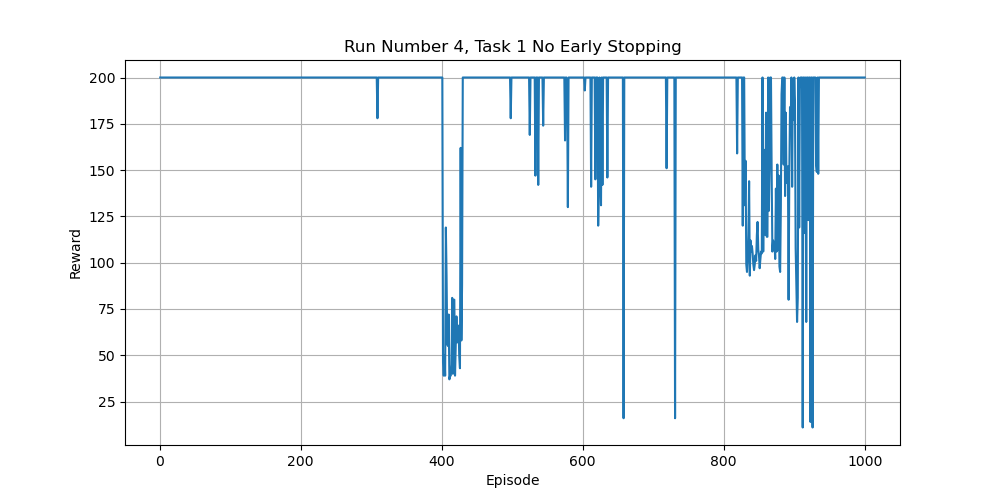
\includegraphics[width=1\textwidth] {imgs/no_early_stopping/Task_1_run_4_no_es} 
        \caption{No Early Stopping for Task 1 (1000 episodes)}
    \end{subfigure} 
         \begin{subfigure}{.45\textwidth}
        \centering
        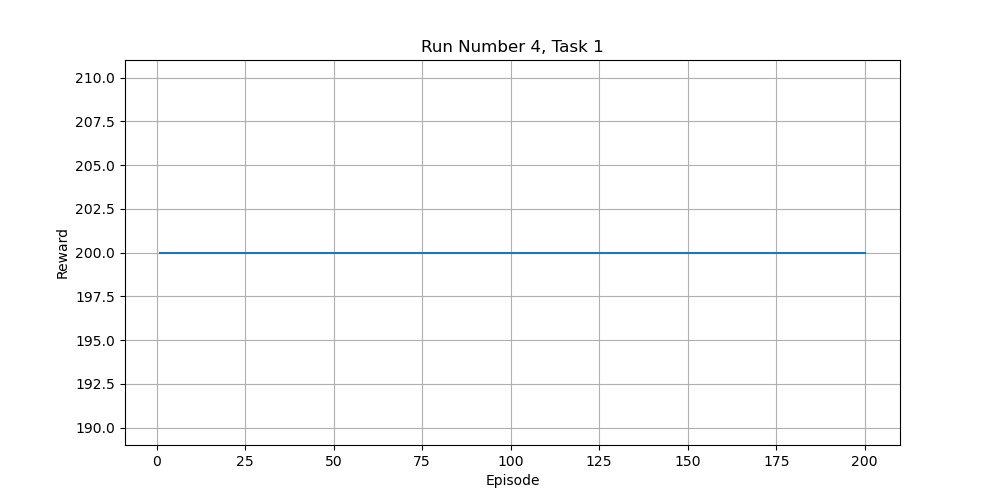
\includegraphics[width=1\textwidth] {imgs/1000_episodes/Task_1_run_4}
        \caption{Early Stopping for Task 1 (exited after 200 episodes)}
    \end{subfigure}
    \end{figure}

\subsection{Few-Shot Learning Validation Metrics}

 \begin{figure}[H]
   \centering
      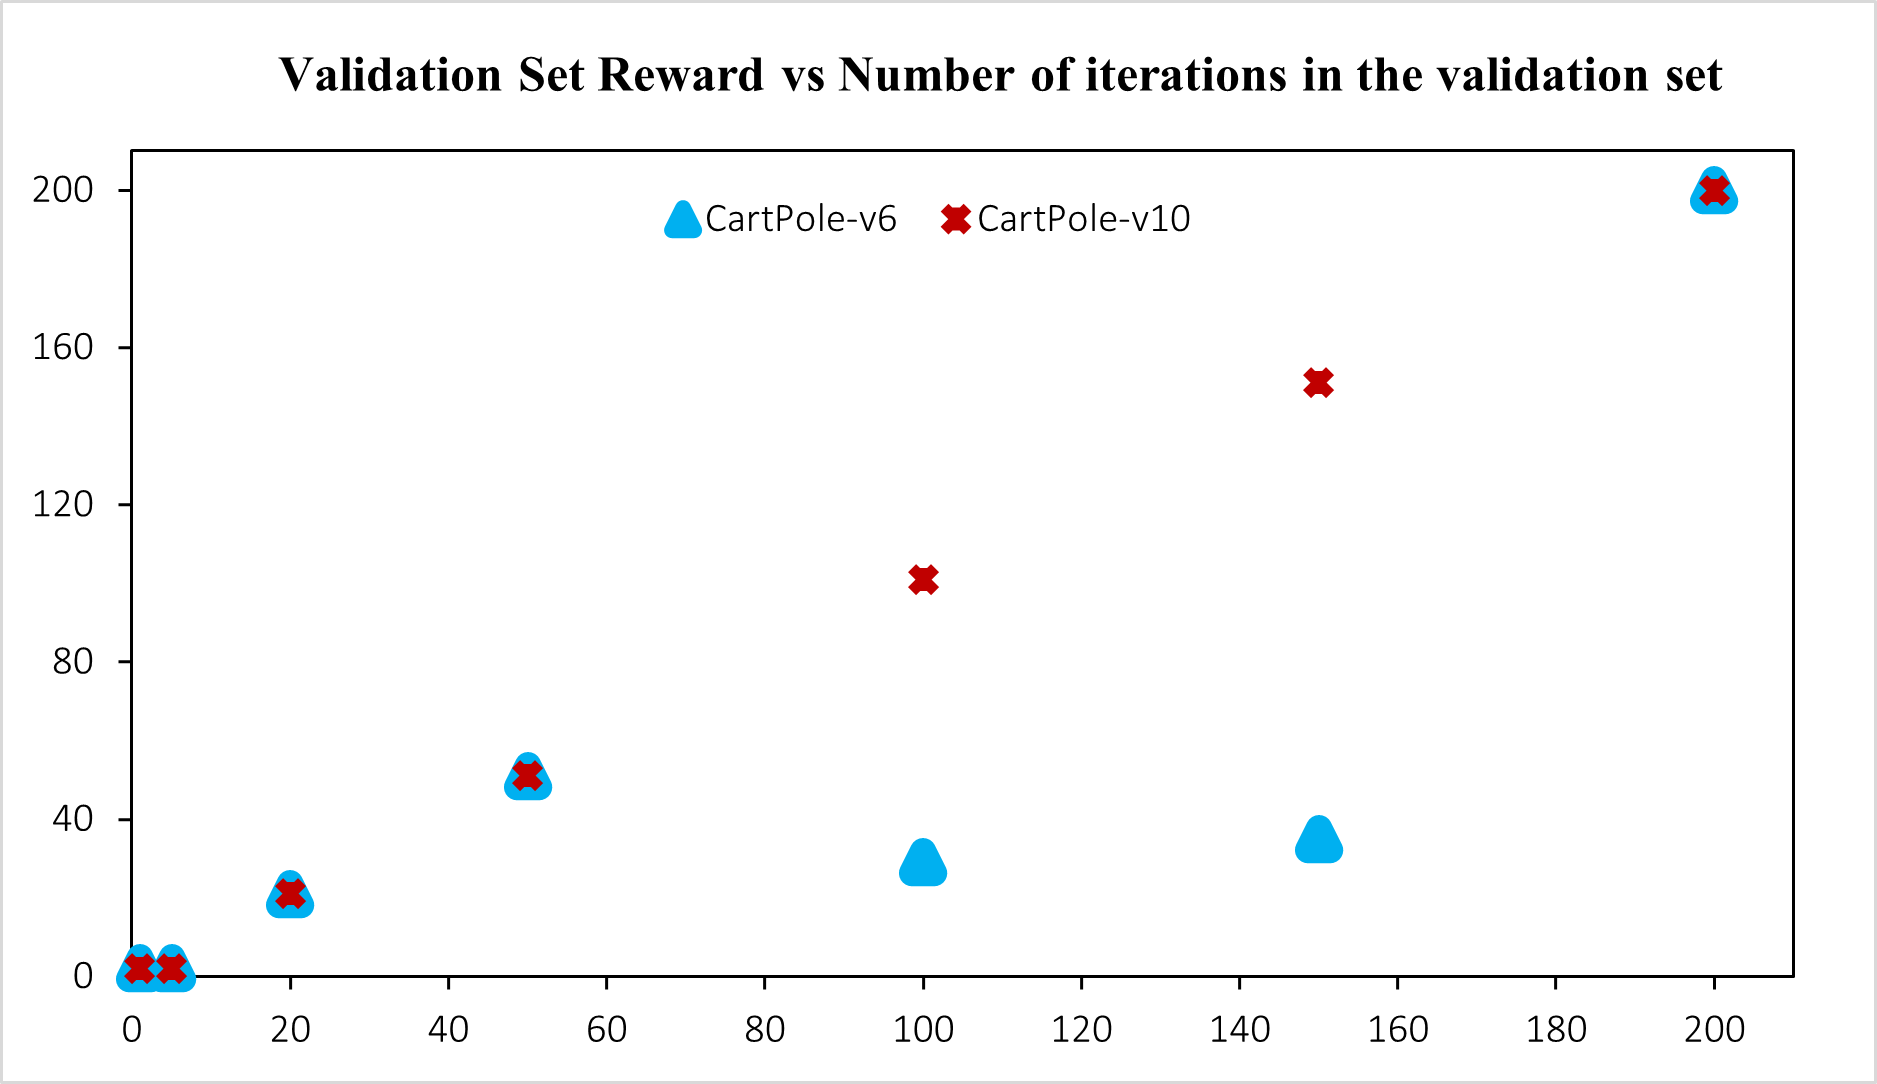
\includegraphics[scale=0.6]{validation_reward}
       \caption{Data table and plot of validation set rewards}
 \end{figure}
 
\begin{table}[h]
\centering
\begin{tabular}{lllllllll}
 &  &  &  & \multicolumn{5}{l}{Number of Gradient Steps (k)}  \\ \cline{3-9} 
 &
  \multicolumn{1}{l|}{} &
  \multicolumn{1}{l|}{1} &
  \multicolumn{1}{l|}{5} &
  \multicolumn{1}{r|}{20} &
  \multicolumn{1}{l|}{50} &
  \multicolumn{1}{r|}{100} &
  \multicolumn{1}{l|}{150} &
  \multicolumn{1}{r|}{200} \\ \cline{2-9} 
\multicolumn{1}{l|}{Validation} &
  \multicolumn{1}{l|}{CartPole-v6} &
  \multicolumn{1}{l|}{2} &
  \multicolumn{1}{l|}{2} &
  \multicolumn{1}{r|}{21} &
  \multicolumn{1}{r|}{51} &
  \multicolumn{1}{r|}{29} &
  \multicolumn{1}{r|}{35} &
  \multicolumn{1}{r|}{200} \\ \cline{2-9} 
\multicolumn{1}{l|}{Environment} &
  \multicolumn{1}{l|}{CartPole-v10} &
  \multicolumn{1}{l|}{2} &
  \multicolumn{1}{l|}{2} &
  \multicolumn{1}{r|}{21} &
  \multicolumn{1}{r|}{51} &
  \multicolumn{1}{r|}{101} &
  \multicolumn{1}{r|}{151} &
  \multicolumn{1}{r|}{200} \\ \cline{2-9} 
\end{tabular}
\end{table}

\noindent A key observation is that the best possible reward of 200 on the validation tasks is only achieved when we let the validation task train for the full 200 gradient steps, comparable to the number of steps we ran the training set tasks. Thus, the number of gradient steps $k$ still is very important to generalization, even with few training examples. 

We believe this under-performance for few-shot learning could be caused either by: (1) our neural network not being complex enough to capture the underlying dynamics which are constant across the training tasks, such as how gravity impacts the pole, or how the mass of the pole impacts dynamics, or (2) the tasks that we chose not having enough similarities. The former is more likely than the latter, as the tasks only had one parameter change.

In cases where the real-world situation we are deploying this model in does not require $100\%$ accuracy, and where speed of deployment is prioritized, this implementation of Reptile would be a good use-case, granted $k$ is chosen to be greater than 20.

\section{Conclusion and Next Steps}
We have evaluated a method for learning a simple RL task which requires 200 gradient steps to learn optimally. Our observations demonstrate that validation task performance scales scale approximately linearly with respect to the number of gradient steps. Our experiments demonstrate that a vanilla implementation of Reptile with $k-$shot learning model on a DQN model is able to train quite well in training-time, but does not generalize well. Even when the tasks were aligned in sequential order, the validation results stayed roughly the same.   Thus, Reptile does not work optimally for very similar CartPole tasks in the Reinforcement Learning domain.


% \newpage

\section{Appendix}

\subsection{Training with 5000 episodes and early stopping}

\begin{figure}[H]
 \centering
 \begin{subfigure}{.45\textwidth}
     \centering
     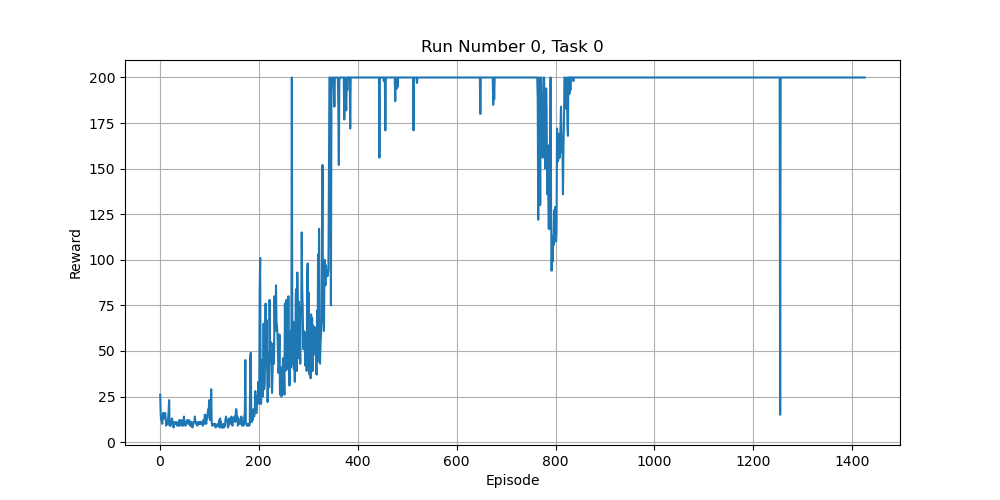
\includegraphics[width=1\textwidth] {imgs/5000_episodes/Task_0_run_0}
 \end{subfigure}%
 \begin{subfigure}{.45\textwidth}
     \centering
     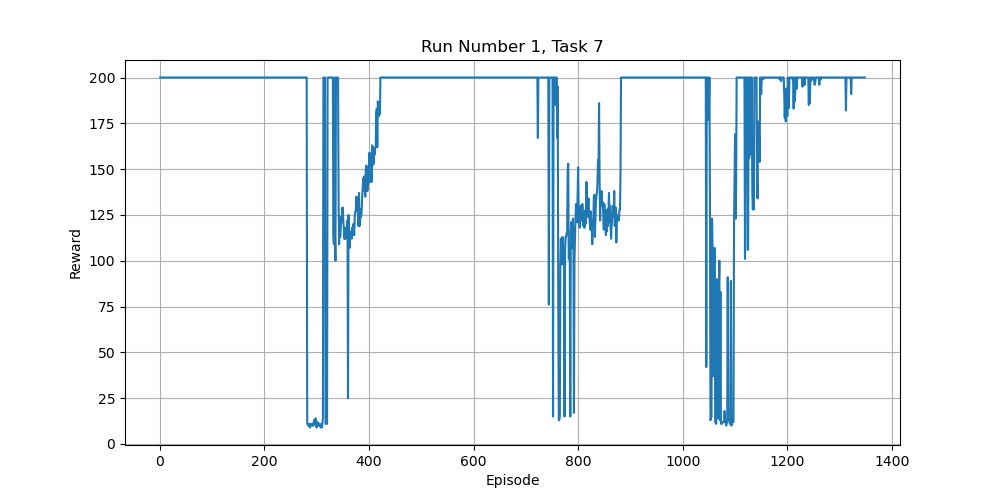
\includegraphics[width=1\textwidth] {imgs/5000_episodes/Task_7_run_1}
 \end{subfigure}
  \begin{subfigure}{.45\textwidth}
      \centering
      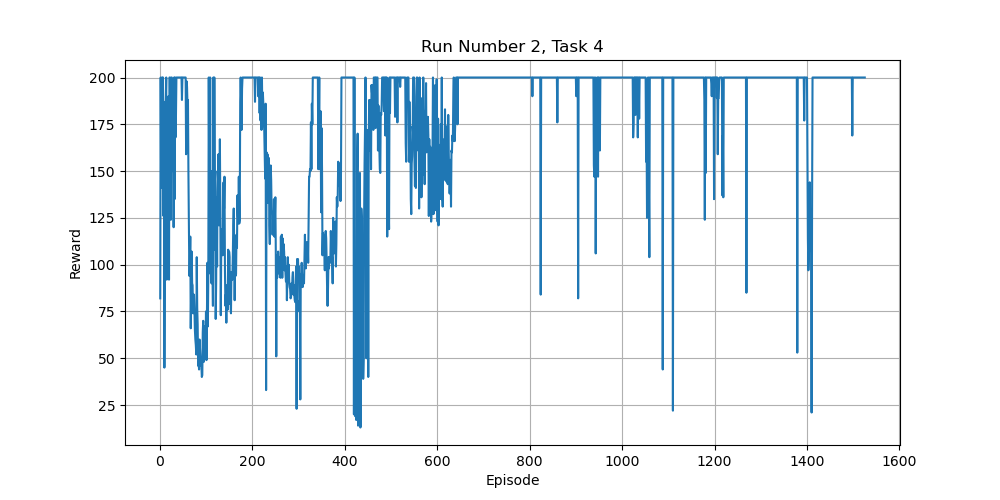
\includegraphics[width=1\textwidth] {imgs/5000_episodes/Task_4_run_2}
  \end{subfigure}
   \begin{subfigure}{.45\textwidth}
       \centering
       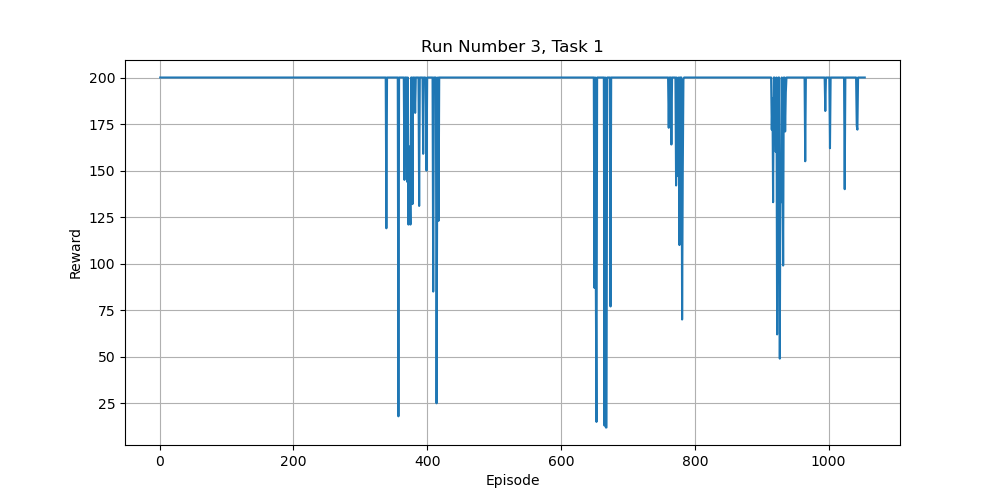
\includegraphics[width=1\textwidth] {imgs/5000_episodes/Task_1_run_3}
   \end{subfigure}
    \begin{subfigure}{.45\textwidth}
        \centering
        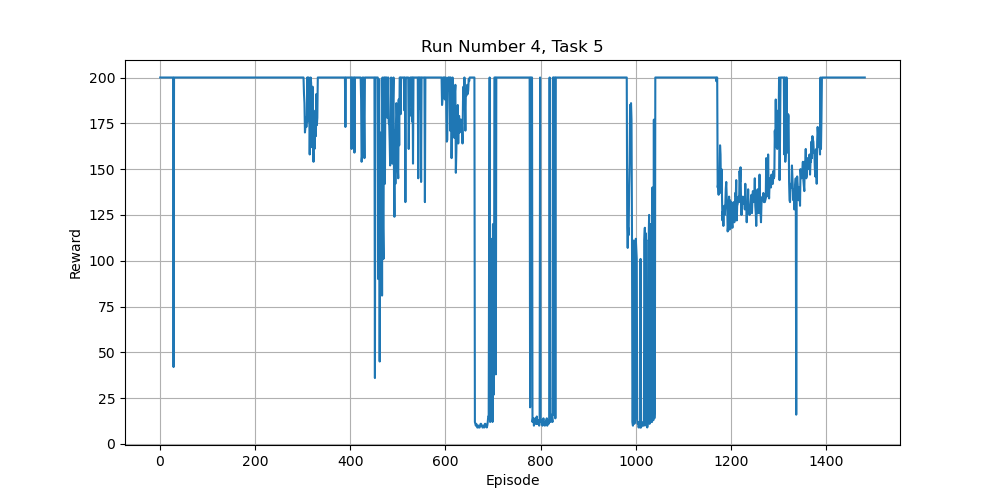
\includegraphics[width=1\textwidth] {imgs/5000_episodes/Task_5_run_4}
    \end{subfigure}
     \begin{subfigure}{.45\textwidth}
         \centering
         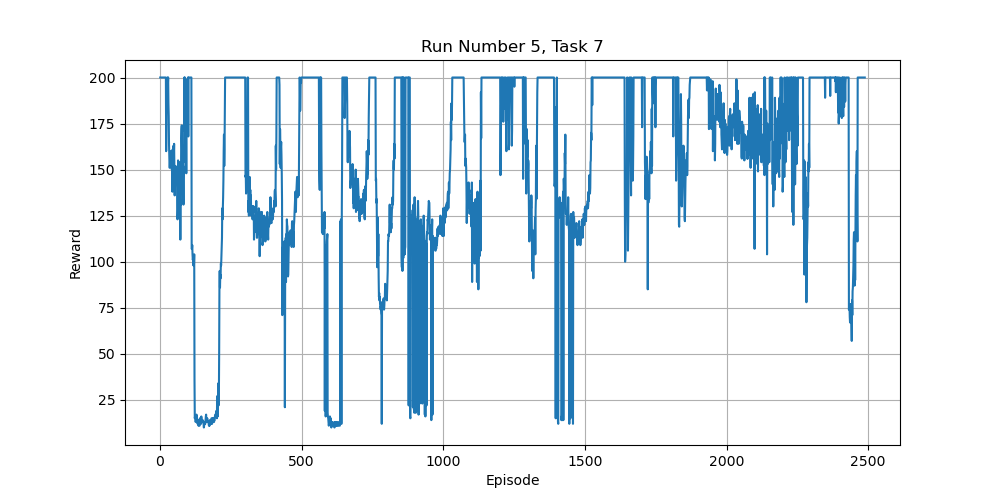
\includegraphics[width=1\textwidth] {imgs/5000_episodes/Task_7_run_5}
     \end{subfigure}
      \begin{subfigure}{.45\textwidth}
          \centering
          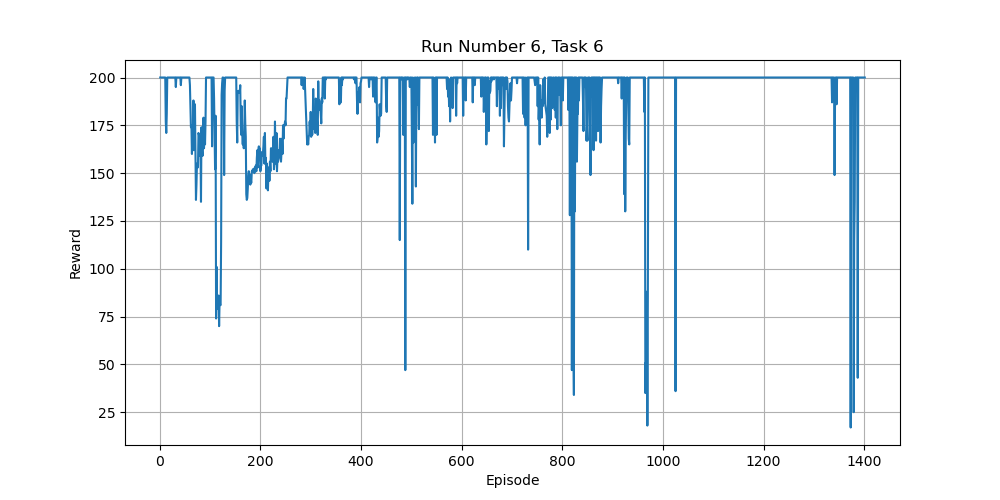
\includegraphics[width=1\textwidth] {imgs/5000_episodes/Task_6_run_6}
      \end{subfigure}
      \begin{subfigure}{.45\textwidth}
          \centering
          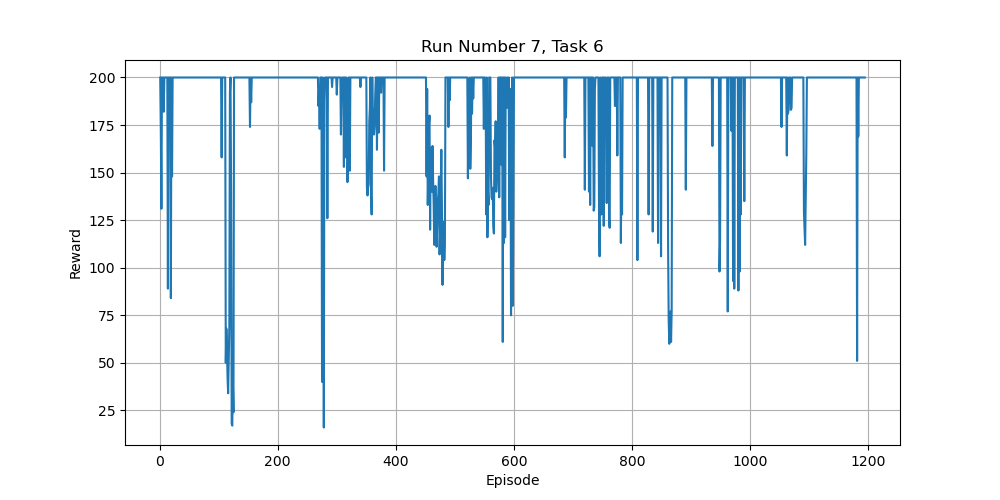
\includegraphics[width=1\textwidth] {imgs/5000_episodes/Task_6_run_7}
      \end{subfigure}
 \end{figure}

\newpage

\subsection{Training with 1000 episodes and early stopping}

\begin{figure}[H]
 \centering
 \begin{subfigure}{.45\textwidth}
     \centering
     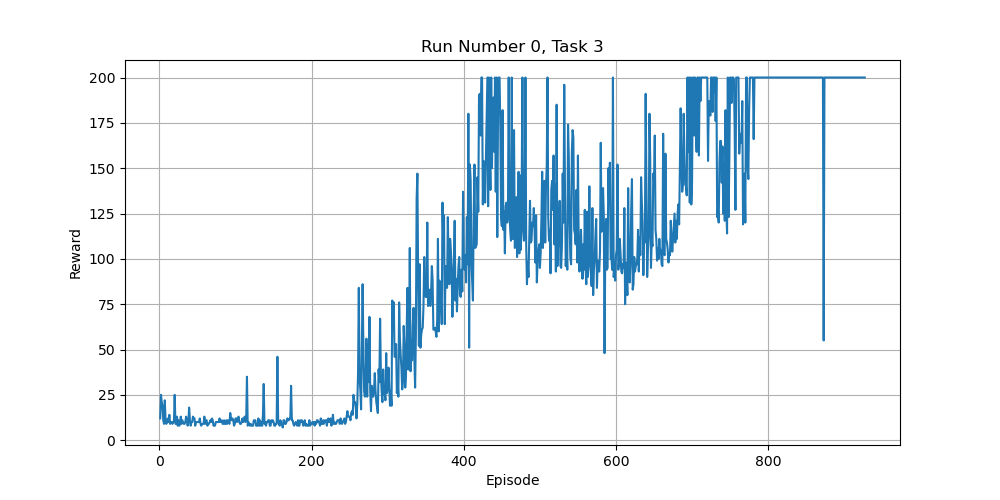
\includegraphics[width=1\textwidth] {imgs/1000_episodes/Task_3_run_0}
 \end{subfigure}%
 \begin{subfigure}{.45\textwidth}
     \centering
     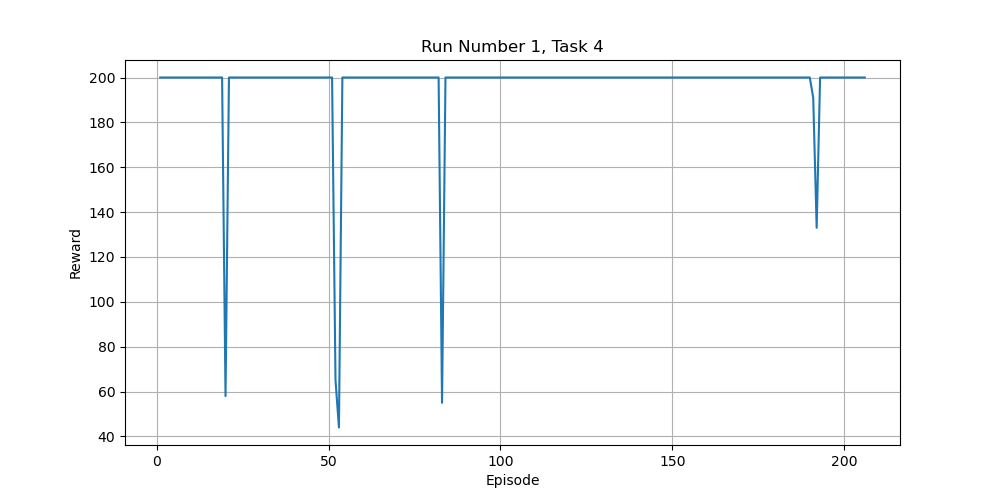
\includegraphics[width=1\textwidth] {imgs/1000_episodes/Task_4_run_1}
 \end{subfigure}
  \begin{subfigure}{.45\textwidth}
      \centering
      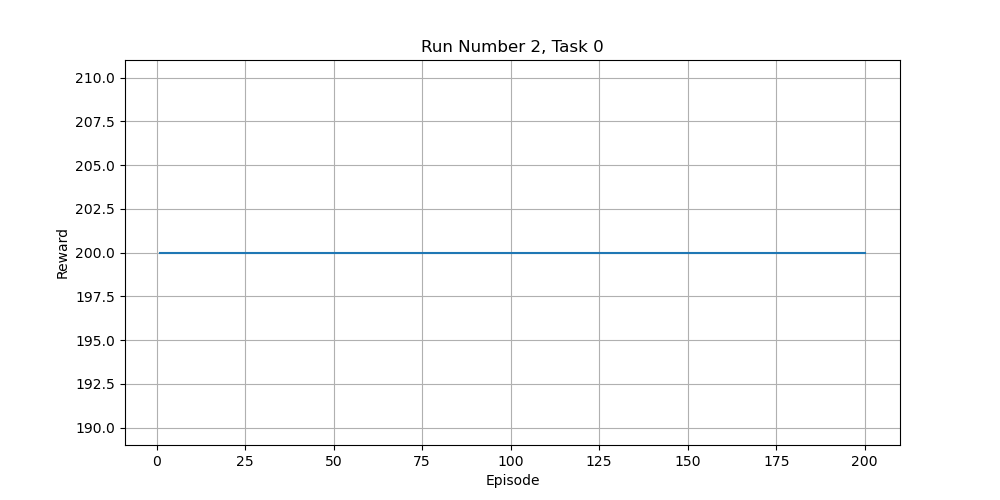
\includegraphics[width=1\textwidth] {imgs/1000_episodes/Task_0_run_2}
  \end{subfigure}
   \begin{subfigure}{.45\textwidth}
       \centering
       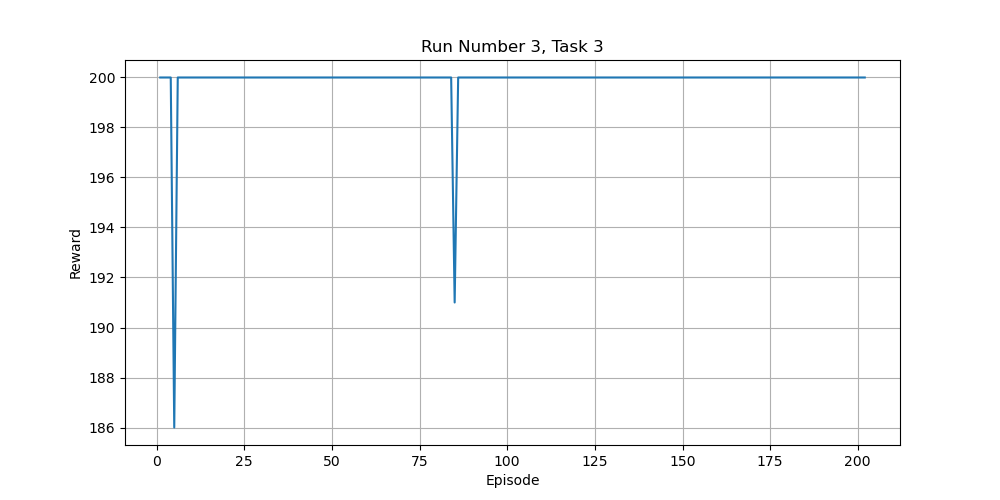
\includegraphics[width=1\textwidth] {imgs/1000_episodes/Task_3_run_3}
   \end{subfigure}
    \begin{subfigure}{.45\textwidth}
        \centering
        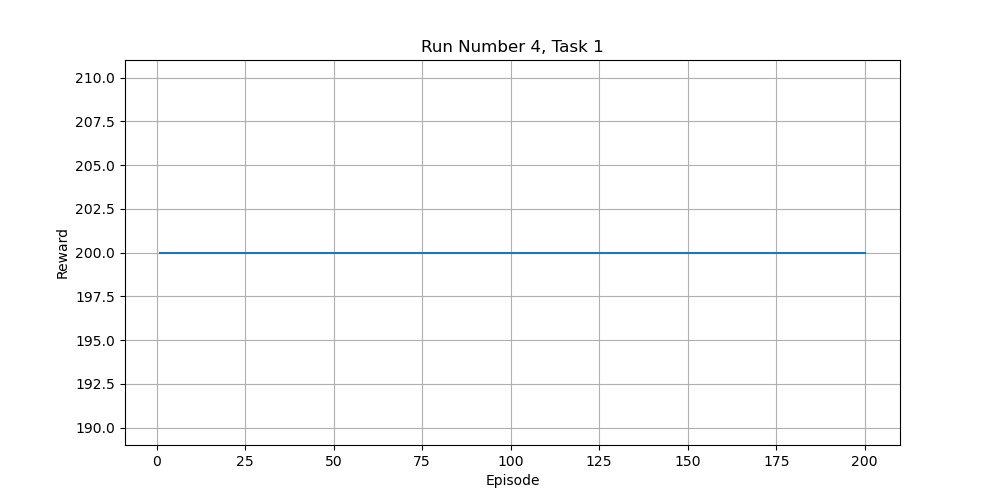
\includegraphics[width=1\textwidth] {imgs/1000_episodes/Task_1_run_4}
    \end{subfigure}
     \begin{subfigure}{.45\textwidth}
         \centering
         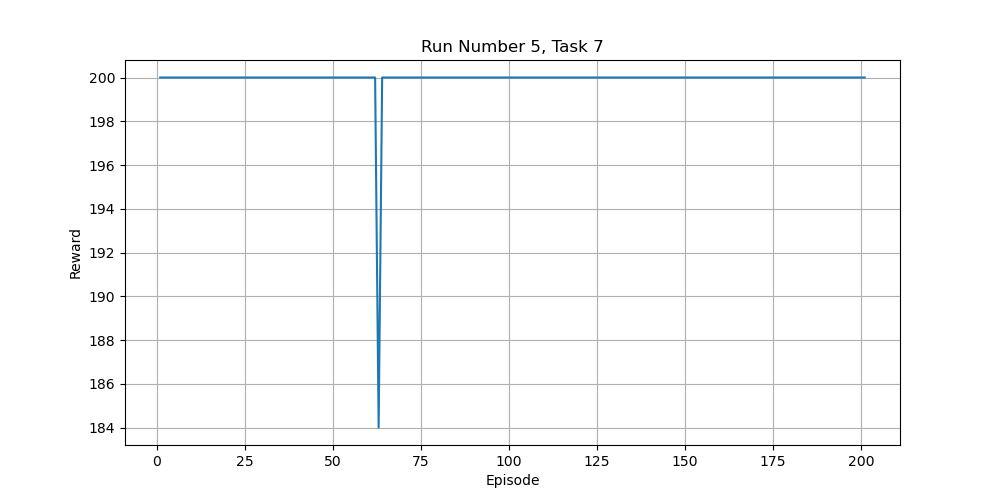
\includegraphics[width=1\textwidth] {imgs/1000_episodes/Task_7_run_5}
     \end{subfigure}
      \begin{subfigure}{.45\textwidth}
          \centering
          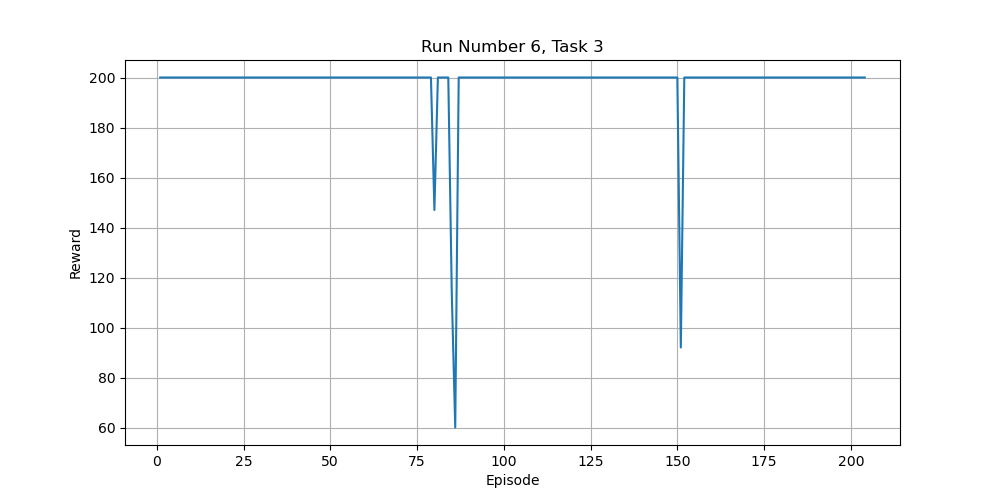
\includegraphics[width=1\textwidth] {imgs/1000_episodes/Task_3_run_6}
      \end{subfigure}
      \begin{subfigure}{.45\textwidth}
          \centering
          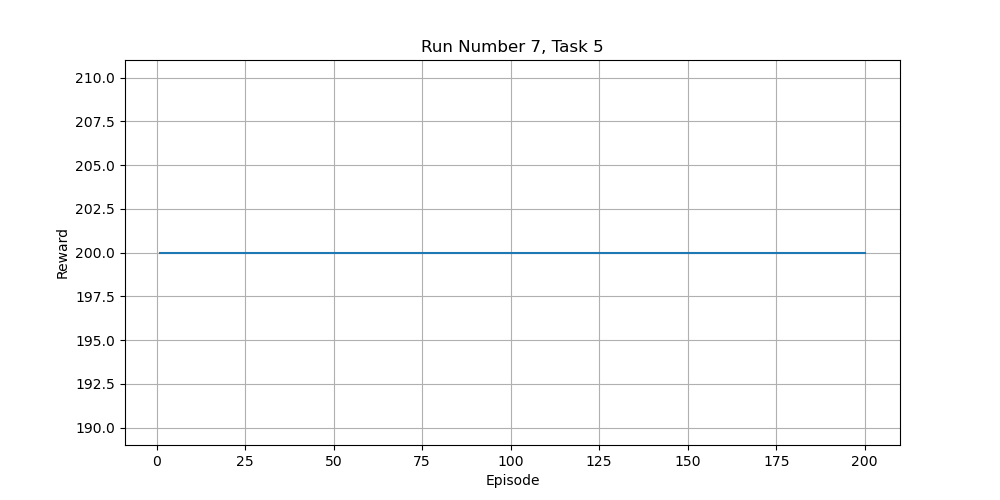
\includegraphics[width=1\textwidth] {imgs/1000_episodes/Task_5_run_7}
      \end{subfigure}
 \end{figure}

\newpage

\subsection{Training with 1000 episodes without early stopping}

\begin{figure}[H]
 \centering
 \begin{subfigure}{.45\textwidth}
     \centering
     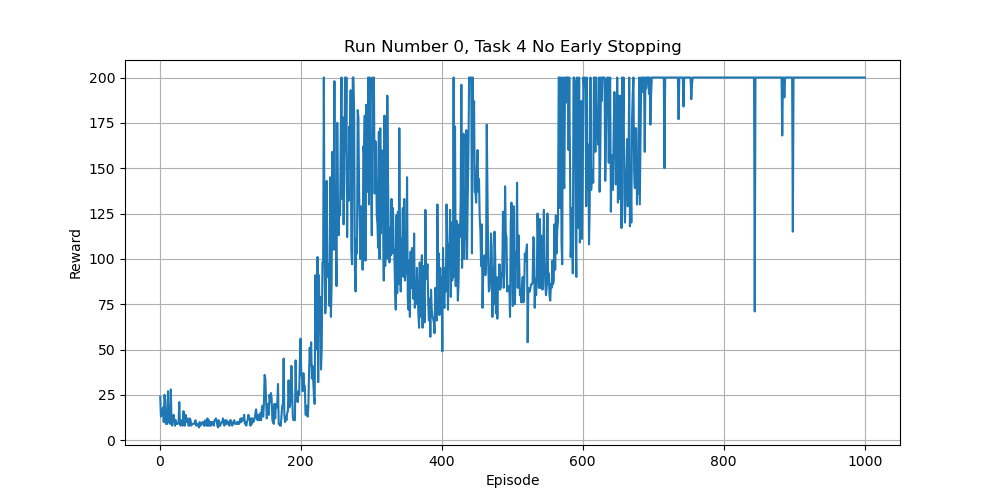
\includegraphics[width=1\textwidth] {imgs/no_early_stopping/Task_4_run_0_no_es}
 \end{subfigure}%
 \begin{subfigure}{.45\textwidth}
     \centering
     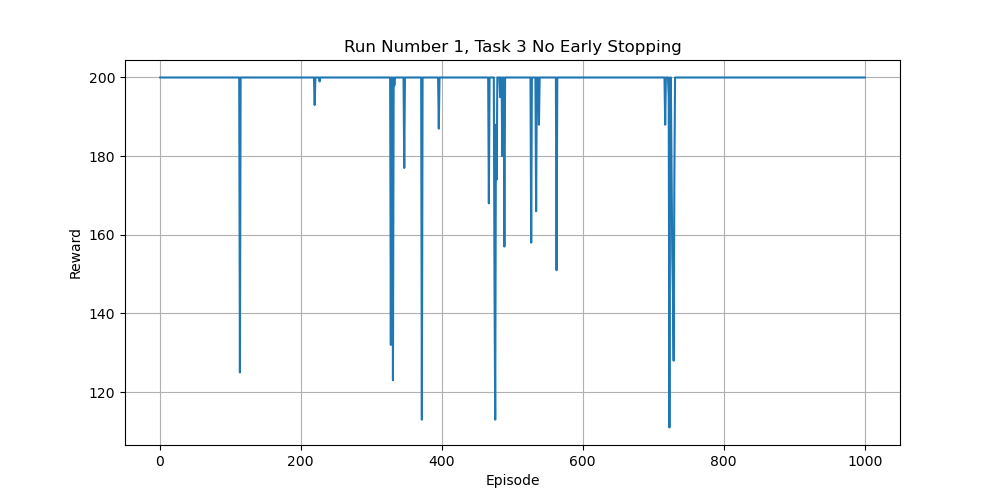
\includegraphics[width=1\textwidth] {imgs/no_early_stopping/Task_3_run_1_no_es}
 \end{subfigure}
  \begin{subfigure}{.45\textwidth}
      \centering
      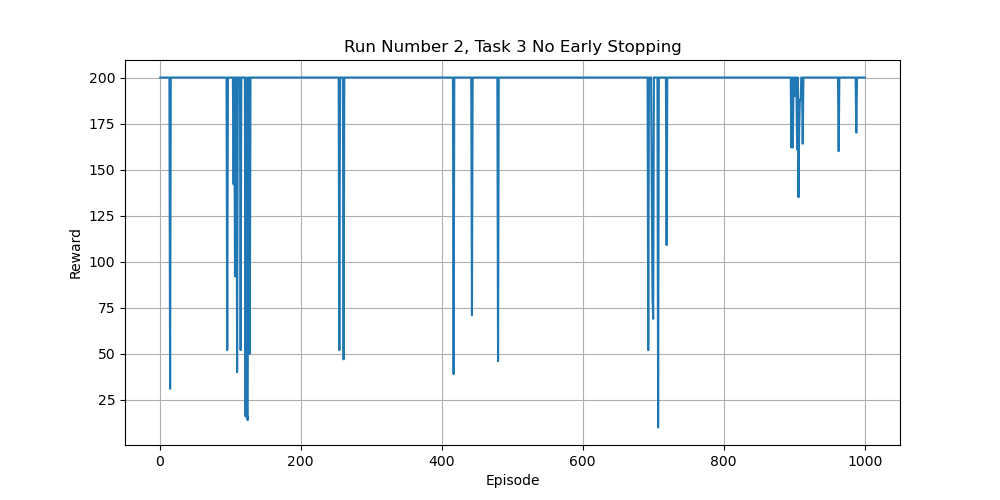
\includegraphics[width=1\textwidth] {imgs/no_early_stopping/Task_3_run_2_no_es}
  \end{subfigure}
   \begin{subfigure}{.45\textwidth}
       \centering
       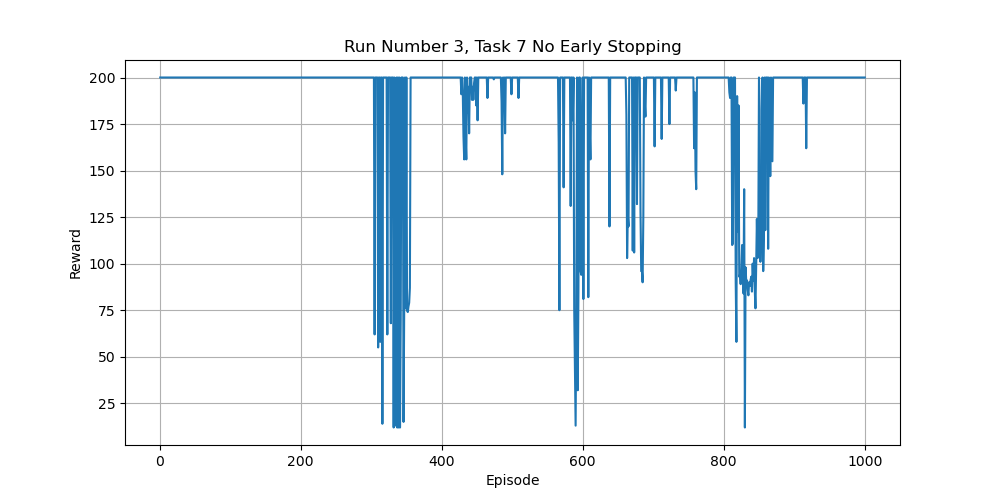
\includegraphics[width=1\textwidth] {imgs/no_early_stopping/Task_7_run_3_no_es}
   \end{subfigure}
    \begin{subfigure}{.45\textwidth}
        \centering
        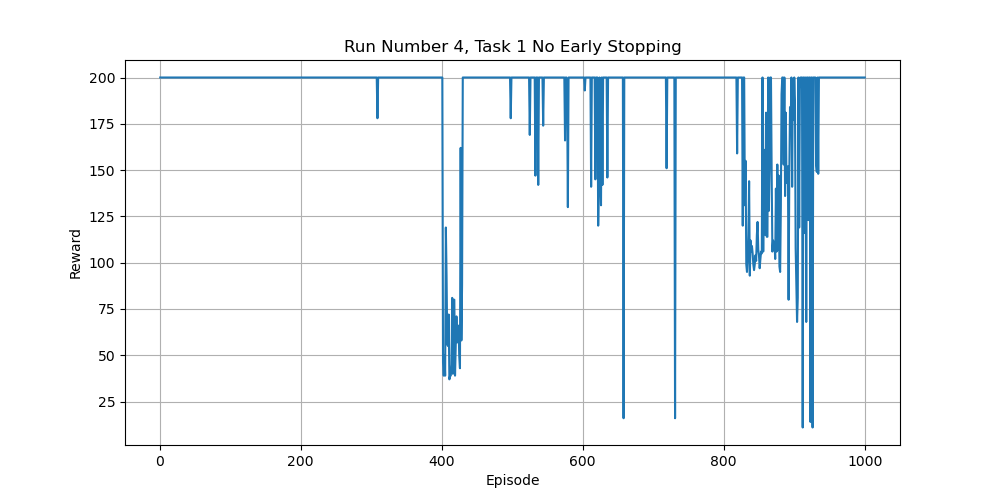
\includegraphics[width=1\textwidth] {imgs/no_early_stopping/Task_1_run_4_no_es}
    \end{subfigure}
     \begin{subfigure}{.45\textwidth}
         \centering
         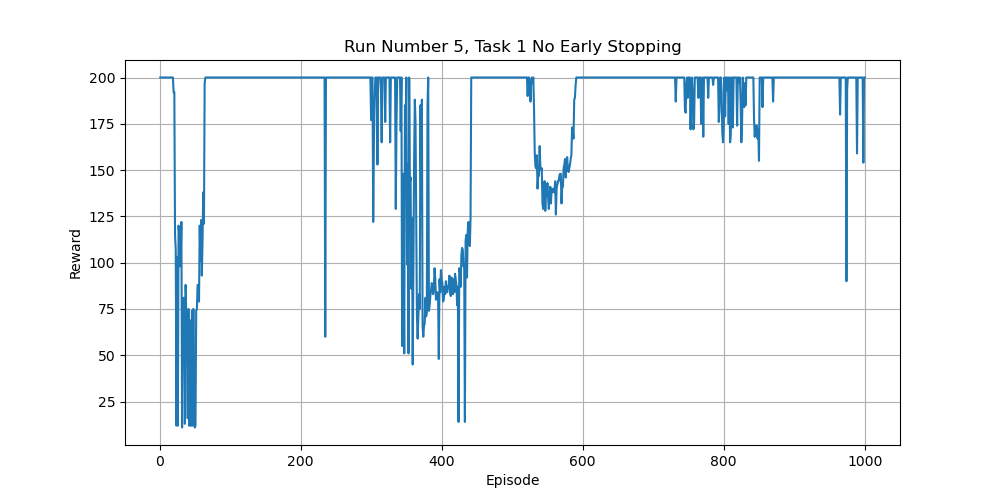
\includegraphics[width=1\textwidth] {imgs/no_early_stopping/Task_1_run_5_no_es}
     \end{subfigure}
      \begin{subfigure}{.45\textwidth}
          \centering
          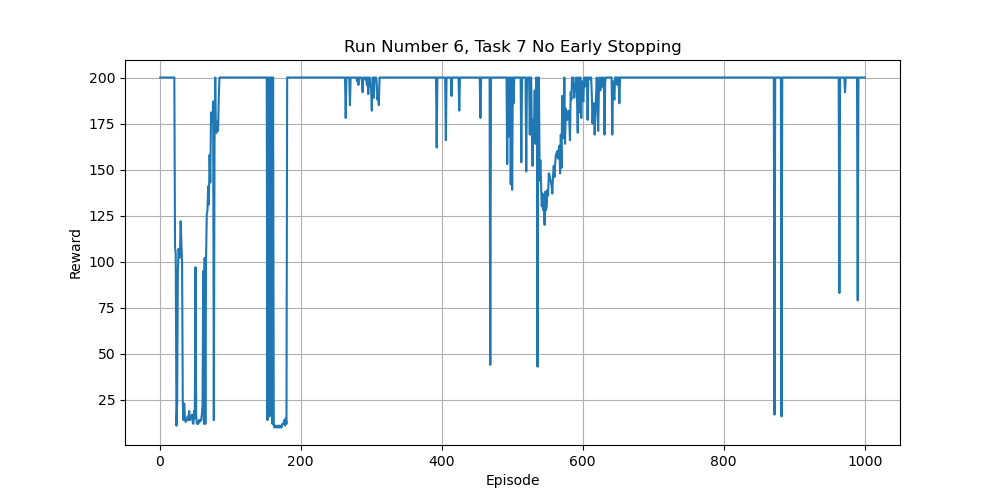
\includegraphics[width=1\textwidth] {imgs/no_early_stopping/Task_7_run_6_no_es}
      \end{subfigure}
      \begin{subfigure}{.45\textwidth}
          \centering
          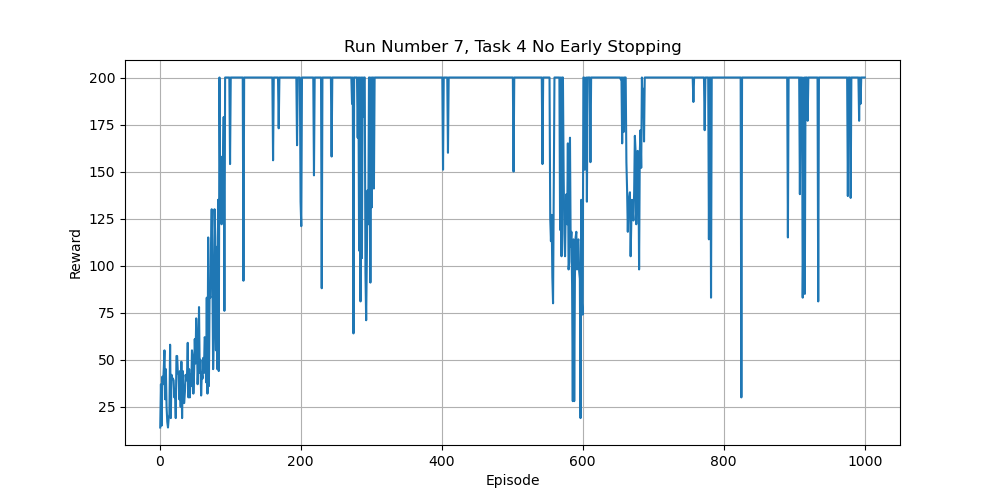
\includegraphics[width=1\textwidth] {imgs/no_early_stopping/Task_4_run_7_no_es}
      \end{subfigure}
 \end{figure}
 
\bibliography{refs}
\bibliographystyle{splncs04}


\end{document}